% Options for packages loaded elsewhere
\PassOptionsToPackage{unicode}{hyperref}
\PassOptionsToPackage{hyphens}{url}
\PassOptionsToPackage{dvipsnames,svgnames,x11names}{xcolor}
%
\documentclass[
  letterpaper,
  DIV=11,
  numbers=noendperiod]{scrartcl}

\usepackage{amsmath,amssymb}
\usepackage{iftex}
\ifPDFTeX
  \usepackage[T1]{fontenc}
  \usepackage[utf8]{inputenc}
  \usepackage{textcomp} % provide euro and other symbols
\else % if luatex or xetex
  \usepackage{unicode-math}
  \defaultfontfeatures{Scale=MatchLowercase}
  \defaultfontfeatures[\rmfamily]{Ligatures=TeX,Scale=1}
\fi
\usepackage{lmodern}
\ifPDFTeX\else  
    % xetex/luatex font selection
\fi
% Use upquote if available, for straight quotes in verbatim environments
\IfFileExists{upquote.sty}{\usepackage{upquote}}{}
\IfFileExists{microtype.sty}{% use microtype if available
  \usepackage[]{microtype}
  \UseMicrotypeSet[protrusion]{basicmath} % disable protrusion for tt fonts
}{}
\makeatletter
\@ifundefined{KOMAClassName}{% if non-KOMA class
  \IfFileExists{parskip.sty}{%
    \usepackage{parskip}
  }{% else
    \setlength{\parindent}{0pt}
    \setlength{\parskip}{6pt plus 2pt minus 1pt}}
}{% if KOMA class
  \KOMAoptions{parskip=half}}
\makeatother
\usepackage{xcolor}
\setlength{\emergencystretch}{3em} % prevent overfull lines
\setcounter{secnumdepth}{-\maxdimen} % remove section numbering
% Make \paragraph and \subparagraph free-standing
\makeatletter
\ifx\paragraph\undefined\else
  \let\oldparagraph\paragraph
  \renewcommand{\paragraph}{
    \@ifstar
      \xxxParagraphStar
      \xxxParagraphNoStar
  }
  \newcommand{\xxxParagraphStar}[1]{\oldparagraph*{#1}\mbox{}}
  \newcommand{\xxxParagraphNoStar}[1]{\oldparagraph{#1}\mbox{}}
\fi
\ifx\subparagraph\undefined\else
  \let\oldsubparagraph\subparagraph
  \renewcommand{\subparagraph}{
    \@ifstar
      \xxxSubParagraphStar
      \xxxSubParagraphNoStar
  }
  \newcommand{\xxxSubParagraphStar}[1]{\oldsubparagraph*{#1}\mbox{}}
  \newcommand{\xxxSubParagraphNoStar}[1]{\oldsubparagraph{#1}\mbox{}}
\fi
\makeatother

\usepackage{color}
\usepackage{fancyvrb}
\newcommand{\VerbBar}{|}
\newcommand{\VERB}{\Verb[commandchars=\\\{\}]}
\DefineVerbatimEnvironment{Highlighting}{Verbatim}{commandchars=\\\{\}}
% Add ',fontsize=\small' for more characters per line
\usepackage{framed}
\definecolor{shadecolor}{RGB}{241,243,245}
\newenvironment{Shaded}{\begin{snugshade}}{\end{snugshade}}
\newcommand{\AlertTok}[1]{\textcolor[rgb]{0.68,0.00,0.00}{#1}}
\newcommand{\AnnotationTok}[1]{\textcolor[rgb]{0.37,0.37,0.37}{#1}}
\newcommand{\AttributeTok}[1]{\textcolor[rgb]{0.40,0.45,0.13}{#1}}
\newcommand{\BaseNTok}[1]{\textcolor[rgb]{0.68,0.00,0.00}{#1}}
\newcommand{\BuiltInTok}[1]{\textcolor[rgb]{0.00,0.23,0.31}{#1}}
\newcommand{\CharTok}[1]{\textcolor[rgb]{0.13,0.47,0.30}{#1}}
\newcommand{\CommentTok}[1]{\textcolor[rgb]{0.37,0.37,0.37}{#1}}
\newcommand{\CommentVarTok}[1]{\textcolor[rgb]{0.37,0.37,0.37}{\textit{#1}}}
\newcommand{\ConstantTok}[1]{\textcolor[rgb]{0.56,0.35,0.01}{#1}}
\newcommand{\ControlFlowTok}[1]{\textcolor[rgb]{0.00,0.23,0.31}{\textbf{#1}}}
\newcommand{\DataTypeTok}[1]{\textcolor[rgb]{0.68,0.00,0.00}{#1}}
\newcommand{\DecValTok}[1]{\textcolor[rgb]{0.68,0.00,0.00}{#1}}
\newcommand{\DocumentationTok}[1]{\textcolor[rgb]{0.37,0.37,0.37}{\textit{#1}}}
\newcommand{\ErrorTok}[1]{\textcolor[rgb]{0.68,0.00,0.00}{#1}}
\newcommand{\ExtensionTok}[1]{\textcolor[rgb]{0.00,0.23,0.31}{#1}}
\newcommand{\FloatTok}[1]{\textcolor[rgb]{0.68,0.00,0.00}{#1}}
\newcommand{\FunctionTok}[1]{\textcolor[rgb]{0.28,0.35,0.67}{#1}}
\newcommand{\ImportTok}[1]{\textcolor[rgb]{0.00,0.46,0.62}{#1}}
\newcommand{\InformationTok}[1]{\textcolor[rgb]{0.37,0.37,0.37}{#1}}
\newcommand{\KeywordTok}[1]{\textcolor[rgb]{0.00,0.23,0.31}{\textbf{#1}}}
\newcommand{\NormalTok}[1]{\textcolor[rgb]{0.00,0.23,0.31}{#1}}
\newcommand{\OperatorTok}[1]{\textcolor[rgb]{0.37,0.37,0.37}{#1}}
\newcommand{\OtherTok}[1]{\textcolor[rgb]{0.00,0.23,0.31}{#1}}
\newcommand{\PreprocessorTok}[1]{\textcolor[rgb]{0.68,0.00,0.00}{#1}}
\newcommand{\RegionMarkerTok}[1]{\textcolor[rgb]{0.00,0.23,0.31}{#1}}
\newcommand{\SpecialCharTok}[1]{\textcolor[rgb]{0.37,0.37,0.37}{#1}}
\newcommand{\SpecialStringTok}[1]{\textcolor[rgb]{0.13,0.47,0.30}{#1}}
\newcommand{\StringTok}[1]{\textcolor[rgb]{0.13,0.47,0.30}{#1}}
\newcommand{\VariableTok}[1]{\textcolor[rgb]{0.07,0.07,0.07}{#1}}
\newcommand{\VerbatimStringTok}[1]{\textcolor[rgb]{0.13,0.47,0.30}{#1}}
\newcommand{\WarningTok}[1]{\textcolor[rgb]{0.37,0.37,0.37}{\textit{#1}}}

\providecommand{\tightlist}{%
  \setlength{\itemsep}{0pt}\setlength{\parskip}{0pt}}\usepackage{longtable,booktabs,array}
\usepackage{calc} % for calculating minipage widths
% Correct order of tables after \paragraph or \subparagraph
\usepackage{etoolbox}
\makeatletter
\patchcmd\longtable{\par}{\if@noskipsec\mbox{}\fi\par}{}{}
\makeatother
% Allow footnotes in longtable head/foot
\IfFileExists{footnotehyper.sty}{\usepackage{footnotehyper}}{\usepackage{footnote}}
\makesavenoteenv{longtable}
\usepackage{graphicx}
\makeatletter
\def\maxwidth{\ifdim\Gin@nat@width>\linewidth\linewidth\else\Gin@nat@width\fi}
\def\maxheight{\ifdim\Gin@nat@height>\textheight\textheight\else\Gin@nat@height\fi}
\makeatother
% Scale images if necessary, so that they will not overflow the page
% margins by default, and it is still possible to overwrite the defaults
% using explicit options in \includegraphics[width, height, ...]{}
\setkeys{Gin}{width=\maxwidth,height=\maxheight,keepaspectratio}
% Set default figure placement to htbp
\makeatletter
\def\fps@figure{htbp}
\makeatother

\KOMAoption{captions}{tableheading}
\makeatletter
\@ifpackageloaded{caption}{}{\usepackage{caption}}
\AtBeginDocument{%
\ifdefined\contentsname
  \renewcommand*\contentsname{Table of contents}
\else
  \newcommand\contentsname{Table of contents}
\fi
\ifdefined\listfigurename
  \renewcommand*\listfigurename{List of Figures}
\else
  \newcommand\listfigurename{List of Figures}
\fi
\ifdefined\listtablename
  \renewcommand*\listtablename{List of Tables}
\else
  \newcommand\listtablename{List of Tables}
\fi
\ifdefined\figurename
  \renewcommand*\figurename{Figure}
\else
  \newcommand\figurename{Figure}
\fi
\ifdefined\tablename
  \renewcommand*\tablename{Table}
\else
  \newcommand\tablename{Table}
\fi
}
\@ifpackageloaded{float}{}{\usepackage{float}}
\floatstyle{ruled}
\@ifundefined{c@chapter}{\newfloat{codelisting}{h}{lop}}{\newfloat{codelisting}{h}{lop}[chapter]}
\floatname{codelisting}{Listing}
\newcommand*\listoflistings{\listof{codelisting}{List of Listings}}
\makeatother
\makeatletter
\makeatother
\makeatletter
\@ifpackageloaded{caption}{}{\usepackage{caption}}
\@ifpackageloaded{subcaption}{}{\usepackage{subcaption}}
\makeatother

\ifLuaTeX
  \usepackage{selnolig}  % disable illegal ligatures
\fi
\usepackage{bookmark}

\IfFileExists{xurl.sty}{\usepackage{xurl}}{} % add URL line breaks if available
\urlstyle{same} % disable monospaced font for URLs
\hypersetup{
  pdftitle={IBM6520\_HW2},
  pdfauthor={Ricky Woznichak},
  colorlinks=true,
  linkcolor={blue},
  filecolor={Maroon},
  citecolor={Blue},
  urlcolor={Blue},
  pdfcreator={LaTeX via pandoc}}


\title{IBM6520\_HW2}
\author{Ricky Woznichak}
\date{2025-02-18}

\begin{document}
\maketitle


\begin{Shaded}
\begin{Highlighting}[]
\FunctionTok{library}\NormalTok{(fpp3)}
\end{Highlighting}
\end{Shaded}

\begin{verbatim}
Registered S3 method overwritten by 'tsibble':
  method               from 
  as_tibble.grouped_df dplyr
\end{verbatim}

\begin{verbatim}
-- Attaching packages -------------------------------------------- fpp3 1.0.1 --
\end{verbatim}

\begin{verbatim}
v tibble      3.2.1     v tsibble     1.1.6
v dplyr       1.1.4     v tsibbledata 0.4.1
v tidyr       1.3.1     v feasts      0.4.1
v lubridate   1.9.4     v fable       0.4.1
v ggplot2     3.5.1     
\end{verbatim}

\begin{verbatim}
-- Conflicts ------------------------------------------------- fpp3_conflicts --
x lubridate::date()    masks base::date()
x dplyr::filter()      masks stats::filter()
x tsibble::intersect() masks base::intersect()
x tsibble::interval()  masks lubridate::interval()
x dplyr::lag()         masks stats::lag()
x tsibble::setdiff()   masks base::setdiff()
x tsibble::union()     masks base::union()
\end{verbatim}

\section{Add Question}\label{add-question}

\begin{Shaded}
\begin{Highlighting}[]
\DocumentationTok{\#\# United States \#\#}
\NormalTok{global\_economy }\SpecialCharTok{|\textgreater{}}
\FunctionTok{filter}\NormalTok{ (Country }\SpecialCharTok{==} \StringTok{\textquotesingle{}United States\textquotesingle{}}\NormalTok{) }\SpecialCharTok{|\textgreater{}}
\FunctionTok{autoplot}\NormalTok{(GDP)}
\end{Highlighting}
\end{Shaded}

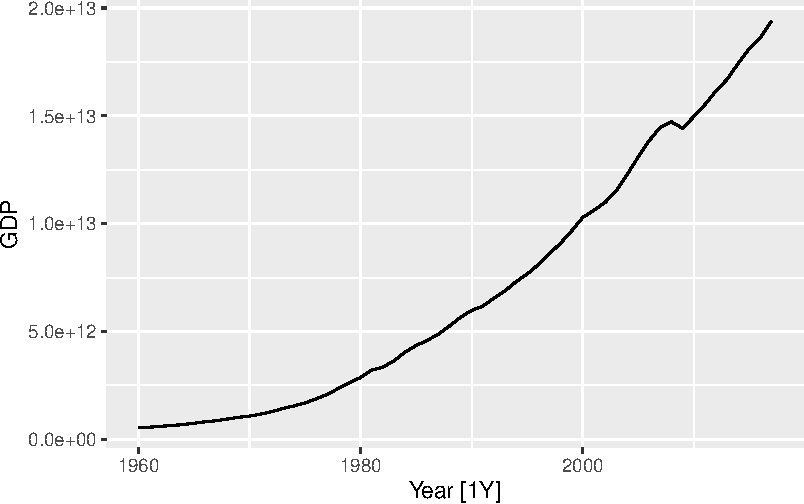
\includegraphics{HW2_IBM6520_files/figure-pdf/unnamed-chunk-2-1.pdf}

\section{Add Question}\label{add-question-1}

\begin{Shaded}
\begin{Highlighting}[]
\DocumentationTok{\#\# Per Capita Adjustments}
\NormalTok{global\_economy }\SpecialCharTok{|\textgreater{}}
\FunctionTok{filter}\NormalTok{ (Country }\SpecialCharTok{==} \StringTok{\textquotesingle{}United States\textquotesingle{}}\NormalTok{) }\SpecialCharTok{|\textgreater{}}
\FunctionTok{autoplot}\NormalTok{(GDP}\SpecialCharTok{/}\NormalTok{ Population) }\SpecialCharTok{+}
\FunctionTok{labs}\NormalTok{(}\AttributeTok{title=} \StringTok{"GDP per capita"}\NormalTok{, }\AttributeTok{y =} \StringTok{"$US"}\NormalTok{)}
\end{Highlighting}
\end{Shaded}

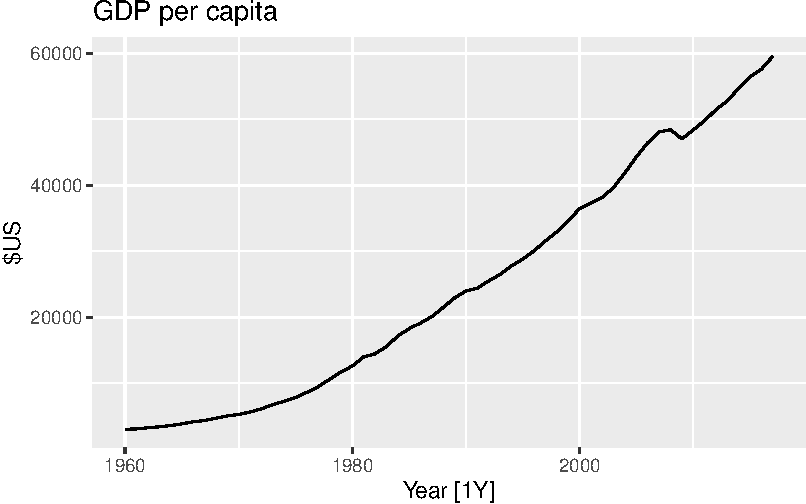
\includegraphics{HW2_IBM6520_files/figure-pdf/unnamed-chunk-3-1.pdf}

\section{Add Question}\label{add-question-2}

\begin{Shaded}
\begin{Highlighting}[]
\NormalTok{aus\_production }\SpecialCharTok{|\textgreater{}}
\FunctionTok{autoplot}\NormalTok{(Gas)}
\end{Highlighting}
\end{Shaded}

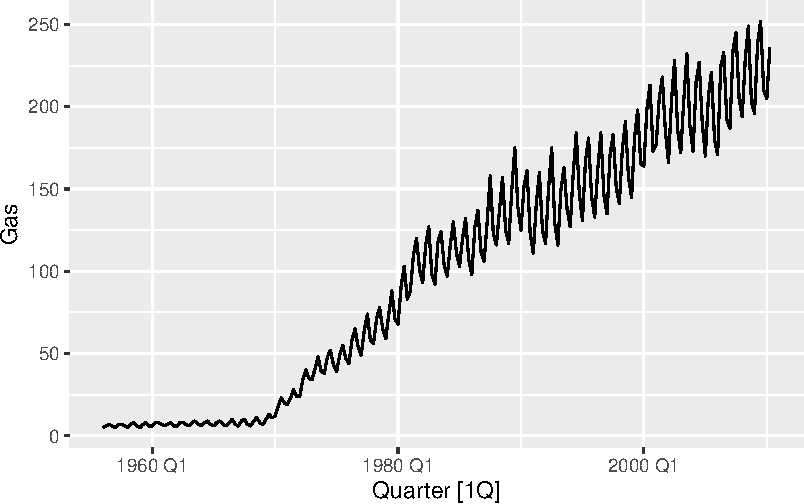
\includegraphics{HW2_IBM6520_files/figure-pdf/unnamed-chunk-4-1.pdf}

\section{Add Question}\label{add-question-3}

\begin{Shaded}
\begin{Highlighting}[]
\NormalTok{lambda }\OtherTok{\textless{}{-}}\NormalTok{ aus\_production }\SpecialCharTok{|\textgreater{}}
\FunctionTok{features}\NormalTok{(Gas, }\AttributeTok{features =}\NormalTok{ guerrero) }\SpecialCharTok{|\textgreater{}}
\FunctionTok{pull}\NormalTok{(lambda\_guerrero)}
\NormalTok{aus\_production }\SpecialCharTok{|\textgreater{}}
\FunctionTok{autoplot}\NormalTok{(}\FunctionTok{box\_cox}\NormalTok{(Gas, lambda)) }\SpecialCharTok{+}
\FunctionTok{labs}\NormalTok{(}\AttributeTok{y =} \StringTok{""}\NormalTok{,}
\AttributeTok{title =} \FunctionTok{paste}\NormalTok{(}\StringTok{"Transformed gas production with lambda = "}\NormalTok{, }\FunctionTok{round}\NormalTok{(lambda,}\DecValTok{2}\NormalTok{)))}
\end{Highlighting}
\end{Shaded}

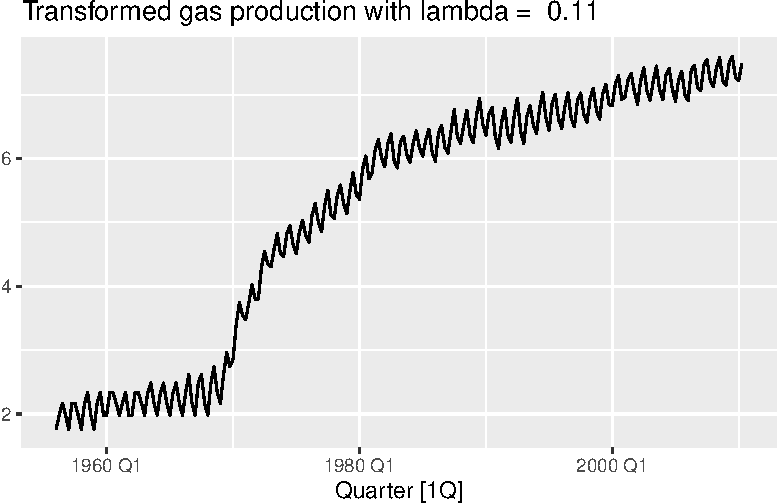
\includegraphics{HW2_IBM6520_files/figure-pdf/unnamed-chunk-5-1.pdf}

\section{Consider the last five years of the Gas data from
aus\_production.}\label{consider-the-last-five-years-of-the-gas-data-from-aus_production.}

\begin{Shaded}
\begin{Highlighting}[]
\NormalTok{gas }\OtherTok{\textless{}{-}} \FunctionTok{tail}\NormalTok{(aus\_production, }\DecValTok{5}\SpecialCharTok{*}\DecValTok{4}\NormalTok{) }\SpecialCharTok{|\textgreater{}} \FunctionTok{select}\NormalTok{(Gas)}
\NormalTok{gas }\SpecialCharTok{|\textgreater{}}
    \FunctionTok{autoplot}\NormalTok{(Gas)}
\end{Highlighting}
\end{Shaded}

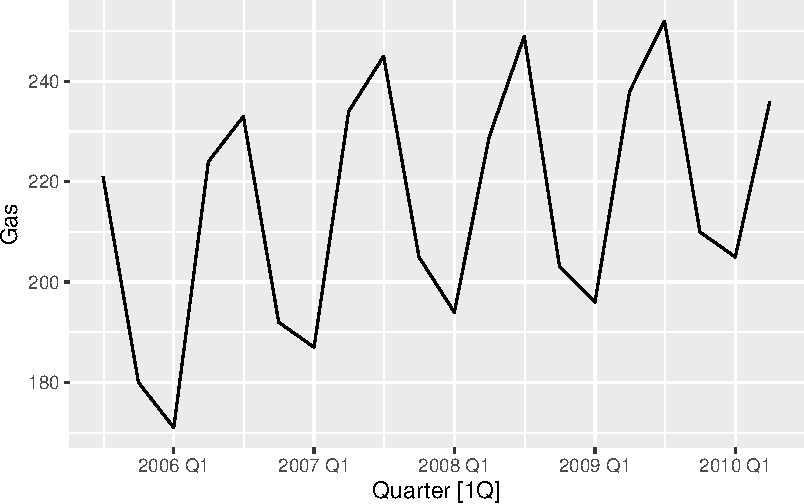
\includegraphics{HW2_IBM6520_files/figure-pdf/unnamed-chunk-6-1.pdf}

\section{b. Use
classical\_decomposition}\label{b.-use-classical_decomposition}

\begin{Shaded}
\begin{Highlighting}[]
\NormalTok{aus\_production }\SpecialCharTok{|\textgreater{}}
\FunctionTok{model}\NormalTok{(}\FunctionTok{classical\_decomposition}\NormalTok{(Gas, }\AttributeTok{type =} \StringTok{"multiplicative"}\NormalTok{)}
\NormalTok{) }\SpecialCharTok{|\textgreater{}}
\FunctionTok{components}\NormalTok{() }\SpecialCharTok{|\textgreater{}}
\FunctionTok{autoplot}\NormalTok{() }\SpecialCharTok{+}
\FunctionTok{labs}\NormalTok{(}\AttributeTok{title =} \StringTok{"Classical additive decomposition of total}
\StringTok{Aus Gas Production"}\NormalTok{)}
\end{Highlighting}
\end{Shaded}

\begin{verbatim}
Warning: Removed 2 rows containing missing values or values outside the scale range
(`geom_line()`).
\end{verbatim}

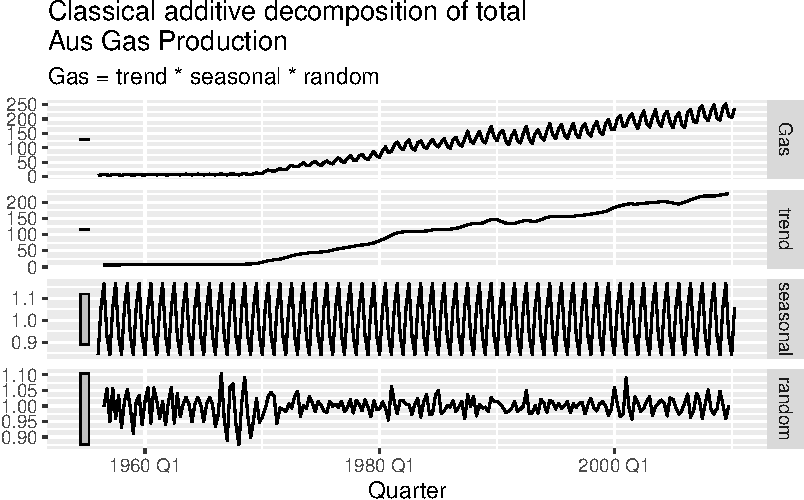
\includegraphics{HW2_IBM6520_files/figure-pdf/unnamed-chunk-7-1.pdf}

\section{c.~Do the results support the graphical interpretation from
part a? (12.5
points)}\label{c.-do-the-results-support-the-graphical-interpretation-from-part-a-12.5-points}

Yes, the result support the upward trend and same seasonal pattern.

\#d.~Compute and plot the seasonally adjusted data. (12.5 points)

\begin{Shaded}
\begin{Highlighting}[]
\NormalTok{dcmp }\OtherTok{\textless{}{-}}\NormalTok{ gas }\SpecialCharTok{|\textgreater{}}
    \FunctionTok{model}\NormalTok{(}\AttributeTok{stl =} \FunctionTok{STL}\NormalTok{(Gas))}
 \FunctionTok{components}\NormalTok{(dcmp) }\SpecialCharTok{|\textgreater{}}
    \FunctionTok{as\_tsibble}\NormalTok{() }\SpecialCharTok{|\textgreater{}}
    \FunctionTok{autoplot}\NormalTok{(Gas, }\AttributeTok{colour =} \StringTok{"red"}\NormalTok{) }\SpecialCharTok{+}
   \FunctionTok{geom\_line}\NormalTok{(}\FunctionTok{aes}\NormalTok{(}\AttributeTok{y=}\NormalTok{season\_adjust), }\AttributeTok{colour =} \StringTok{"blue"}\NormalTok{) }\SpecialCharTok{+}
     \FunctionTok{labs}\NormalTok{(}\AttributeTok{y =} \StringTok{"Gas Production"}\NormalTok{,}
         \AttributeTok{title =} \StringTok{"Seasonally Adjusted Gas Production"}\NormalTok{)}
\end{Highlighting}
\end{Shaded}

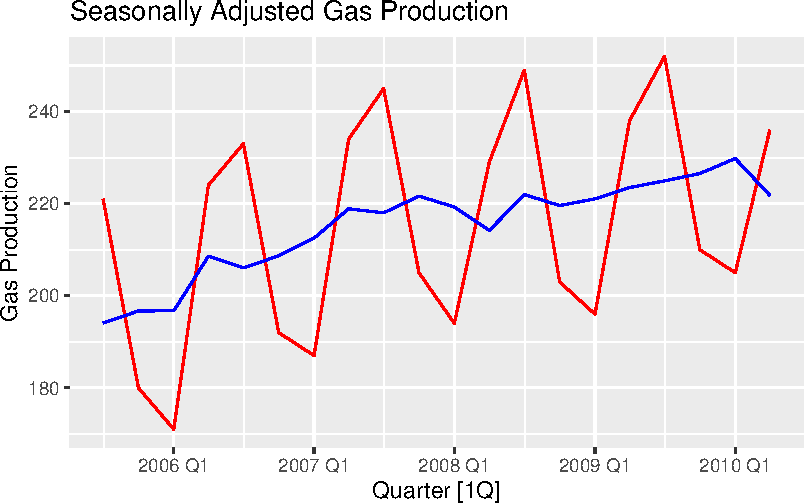
\includegraphics{HW2_IBM6520_files/figure-pdf/unnamed-chunk-8-1.pdf}




\end{document}
